\subsubsection{UC3 - Scelta della visualizzazione}
\begin{figure}[h]
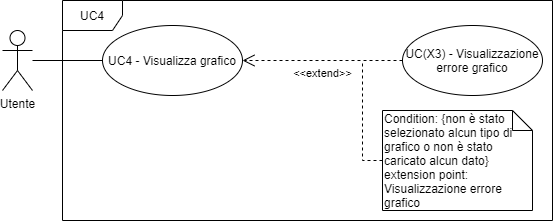
\includegraphics[width=\linewidth]{section/Images/UC5SceltaVisualizzazione.png}
\centering
\caption{UC5 - Scelta della visualizzazione}
\end{figure}
\begin{itemize}
	\item \textbf{Attore primario}: Utente.
	\item \textbf{Precondizioni}: L'utente ha caricato dei dati nel sistema [UC1] e ha selezionato le dimensioni da utilizzare [UC2].
	\item \textbf{Postcondizioni}: Viene mostrata la visualizzazione scelta.
	\item \textbf{Scenario principale}:
		\begin{enumerate}
			\item L'utente seleziona una visualizzazione tra quelle disponibili;
		\end{enumerate}
	\item \textbf{Estensioni}:
	\begin{enumerate}[(a)]
		\item Nel caso in cui non è stato caricato alcun dato o non è stata scelta alcuna dimensione:
		\begin{enumerate}[1.]
			\item il grafico non viene visualizzato;
			\item viene visualizzato un errore esplicativo [UC7.3].
		\end{enumerate}
	\end{enumerate}
\end{itemize}